\chapter{Introdução}
\label{ch:introducao}
\begin{resumocapitulo}
	Este resumo pode ser utilizado para melhorar a comunicação com o leitor. As seções e subseções são configuradas de acordo com a normas ABNT (2020) adotada pela Uninove (tamanho da fonte, espaçamento...). As numerações de página estão alinhadas a direita no cabeçalho. Neste capítulo são mostrados exemplos para utilização de comandos de \textbf{citação}, \textbf{tabelas}, \textbf{quadros}, \textbf{equações} e \textbf{algoritmos}. Para ter acesso a documentação diretamente na biblioteca da Uninove, \href{http://docs.uninove.br/arte/pdfs/Manual_de_Trabalhos_Academicos_ABNT_UNINOVE.pdf}{clique aqui.}
\end{resumocapitulo}

\section{Citações diretas e indiretas}
\label{sec:citacoes}
\subsection{Citação Direta}
\label{subsec:citacao_direta}
O comando \texttt{$\backslash$citeonline\{Referencia-refs.bib\}} gera o seguinte resultado:

Segundo \citeonline{mitchell1997machine}, aprendizagem de máquina ``[...] é como um programa de computador aprende pela experiência \textit{E}, com respeito a algum tipo de tarefa \textit{T} e performance \textit{P}, se sua performance \textit{P} nas tarefas em \textit{T}, na forma medida por \textit{P}, melhoram com a experiência''.

\subsection{Citação Indireta}
\label{subsec:citacao_indireta}
O comando \texttt{$\backslash$cite\{Referencia-refs.bib\}} gera o seguinte resultado:

O SCImago é um portal que fornece indicadores de produções científicas contidas no banco de dados do Scopus \cite{Villasenor-Almaraz2019}, sobre os principais periódicos do mundo \cite{DUggento2016}.

\section{Montagem de Tabela}
\label{sec:tabela}
A seguir o exemplo de uma tabela, Tabela~\ref{tab:tab_identificador}. Para tabelas mais complexas acesse \textbf{Tables Generator} (\href{https://www.tablesgenerator.com/}{https://www.tablesgenerator.com}).
\begin{table}[!ht]
	\centering
	\caption{Descrição da tabela}
	\label{tab:tab_identificador}
	\begin{tabular*}{\columnwidth}{@{\extracolsep{\fill}}lrccc@{}}
		\toprule[1pt]{}\textbf{Desc. 1} & \textbf{Desc. 2} & \textbf{Desc. 4} & \textbf{Desc. 5} & \textbf{Desc. 6}\\\hline
		Item 1		& 901     	& 376  	& 4,738 & 21,317	\\
		Item 2		& 790		& 654  	& 5,913 & 45,540	\\
		Item 3 		& 333		& 215  	& 5,616 & 10,500	\\
		\bottomrule[1pt]
	\end{tabular*}
	\raggedright
	\amostra{2.024} \\% determina o tamanho de uma amostra
	\fontetabela{Autor} % alinha o nome do autor à esquerda
\end{table}

% \begin{landscape}
% 	\begin{table}[!ht]
% 		\small
% 		\centering
% 		\begin{tabular}{llllllllllll}
% 			\hline
% 			\\
% 			\multicolumn{12}{l}{\textbf{Total trade by country and by year (in US\$)}}    \\
% 			\hline \hline
% 			\\
% 			 & 2003 & 2004 & 2005 & 2006 & 2007 & 2008 & 2009 & 2010 & 2011 & 2012 & 2013 \\
% 			...
% 		\end{tabular}
% 		\caption{Trade volume evolution Costa Rica - EFTA}
% 		\label{tbl:tradeevo-costa-efta}
% 	\end{table}
% \end{landscape}


\begin{landscape}
	\begin{table}[!ht]
		\small
		\centering
		\caption{Formatação no modo paisagem para textos grandes.}
		\label{tab:loadings}
		\begin{tabular*}{\columnwidth}{@{\extracolsep{\fill}}lccc@{}}
			\toprule[1pt]{}\textbf{Categories}      & \textbf{Factor 1} & \textbf{Factor 2} & \textbf{Communality}
			\\\hline
			Study Concept           & 0.645		& 0.324   & 0.52	\\
			Study Supervision		& 0.628		& 0.116   & 0.41	\\
			Funding and/or Support  & 0.484		& 0.144   & 0.24	\\
			Critical Revision   	& 0.441		& 0.238   & 0.25	\\
			Study Concept           & 0.645		& 0.324   & 0.52	\\
			Study Supervision		& 0.628		& 0.116   & 0.41	\\
			Funding and/or Support  & 0.484		& 0.144   & 0.24	\\
			Critical Revision   	& 0.441		& 0.238   & 0.25	\\
			Statistical Analysis 	& 0.107		& 0.724  & 0.54		\\
			Original Draft			& 0.338		& 0.525  & 0.38		\\
			Data Collection			& 0.245   	& 0.275  & 0.14		\\
			Statistical Analysis 	& 0.107		& 0.724  & 0.54		\\
			Original Draft			& 0.338		& 0.525  & 0.38		\\
			Data Collection			& 0.245   	& 0.275  & 0.14		\\
			\hline \\[-1.8ex]
			\textit{Cronbach's $\alpha$}	& \textit{0.656}     & \textit{0.550}  \\
			\bottomrule[1pt]
		\end{tabular*}
		\fonte{Autor}
	\end{table}
\end{landscape}

\section{Montagem de Quadro}
\label{sec:quadro}
Os quadros também podem ser posicionados no modo paisagem, conforme as configurações da tabela anterior.

\begin{quadros}[ht!]
	\caption{Descrição dos dados contidos no quadro.}
	\label{quad:contribuicoes_annals}
	\centering
	\begin{small}
		\def\arraystretch{1.1}
		\begin{tabular}{|p{1.0cm}|p{14.0cm}|}
			\hline
			\textbf{\#} & \textbf{Descrição} \\\hline
			1           & \textit{Linha 1}   \\\hline
			2           & \textit{Linha 2}   \\\hline
			3           & \textit{Linha 3}   \\\hline
			4           & \textit{Linha 4}   \\\hline
			5           & \textit{Linha 5}   \\\hline
		\end{tabular}
	\end{small}
	\fonte{\cite{Abbasi2011}}
\end{quadros}

\section{Montagem de Equação}
\label{sec:equacao}
\begin{definicao}{Média aritmética}
	Para uma amostra $ X=\{x_1,, x_2, \ldots,x_n\} $ de observações, onde $ n $ é o número de observações, se define a média aritmética da seguinte forma:
	\begin{equation}
		\mu(X)=\dfrac{1}{n}\sum\limits_{x \in X}x
	\end{equation}
\end{definicao}
\begin{proposicao}
	Se $ k $ é uma constante então multiplicar a média de uma amostra $ X $ é o mesmo de multiplicar cada elemento de $ X $ por $ k $, isto é, $ k \times \mu(X) = \dfrac{1}{n} \sum\limits_{x \in X}x\times k $.
\end{proposicao}
\begin{prova}
	Desenvolve-se a igualdade:
	\begin{align*}
		k \times \mu(X) & = \dfrac{1}{n} \sum\limits_{x \in X}xk                           \\
		                & \Longleftrightarrow  \dfrac{(x_1k,x_2k, \ldots, x_nk)}{n}        \\
		                & \Longleftrightarrow  \dfrac{nk \times (x_1,x_2, \ldots, x_n)}{n} \\
		                & \Longleftrightarrow   k \times \dfrac{(x_1,x_2, \ldots, x_n)}{n} \\
		                & \Longleftrightarrow   k \times \mu(X) \numberequation{1}
	\end{align*}
\end{prova}
Assim, concluí-se que $ k \times \mu(X) = \dfrac{1}{n} \sum\limits_{x \in X}x\times k $.

\section{Montagem de Algoritmo}
\label{sec:algortimo}
Apresentação do Algoritmo~\ref{algorithm:algoritmo_descricao}.
\begin{algorithm}
	\SetInd{0.5cm}{0.1cm}
	\Entrada{$Artigos$}
	\Saida{$Dataset$}
	\SetAlgoLined

	$ Dataset \leftarrow \emptyset $ \\
	\ForEach{$\text{artigo}~i \in \text{Artigos} $}{
		$ autor \leftarrow \emptyset $ \\
		\ForEach{$\text{autor}~k \in \text{artigo} $}{
			$ autor[k] \leftarrow \text{Extrair as informações de um dado~$i$ para o dado~$k$} $ \;
		}
		$ Dataset $ $\leftarrow \text{Adicionar os dados do}~dado $ \;
	}
	\caption{Texto que descreve o algoritmo.}
	\label{algorithm:algoritmo_descricao}
\end{algorithm}

\section{Inclusão de Figura}
\label{sec:figura}
A Figura~\ref{fig:identificador_da_figura} mostra os tipos de estruturação de dados.
\begin{figure}[!ht]
	{\centering
		\caption{Descrição da figura.}
		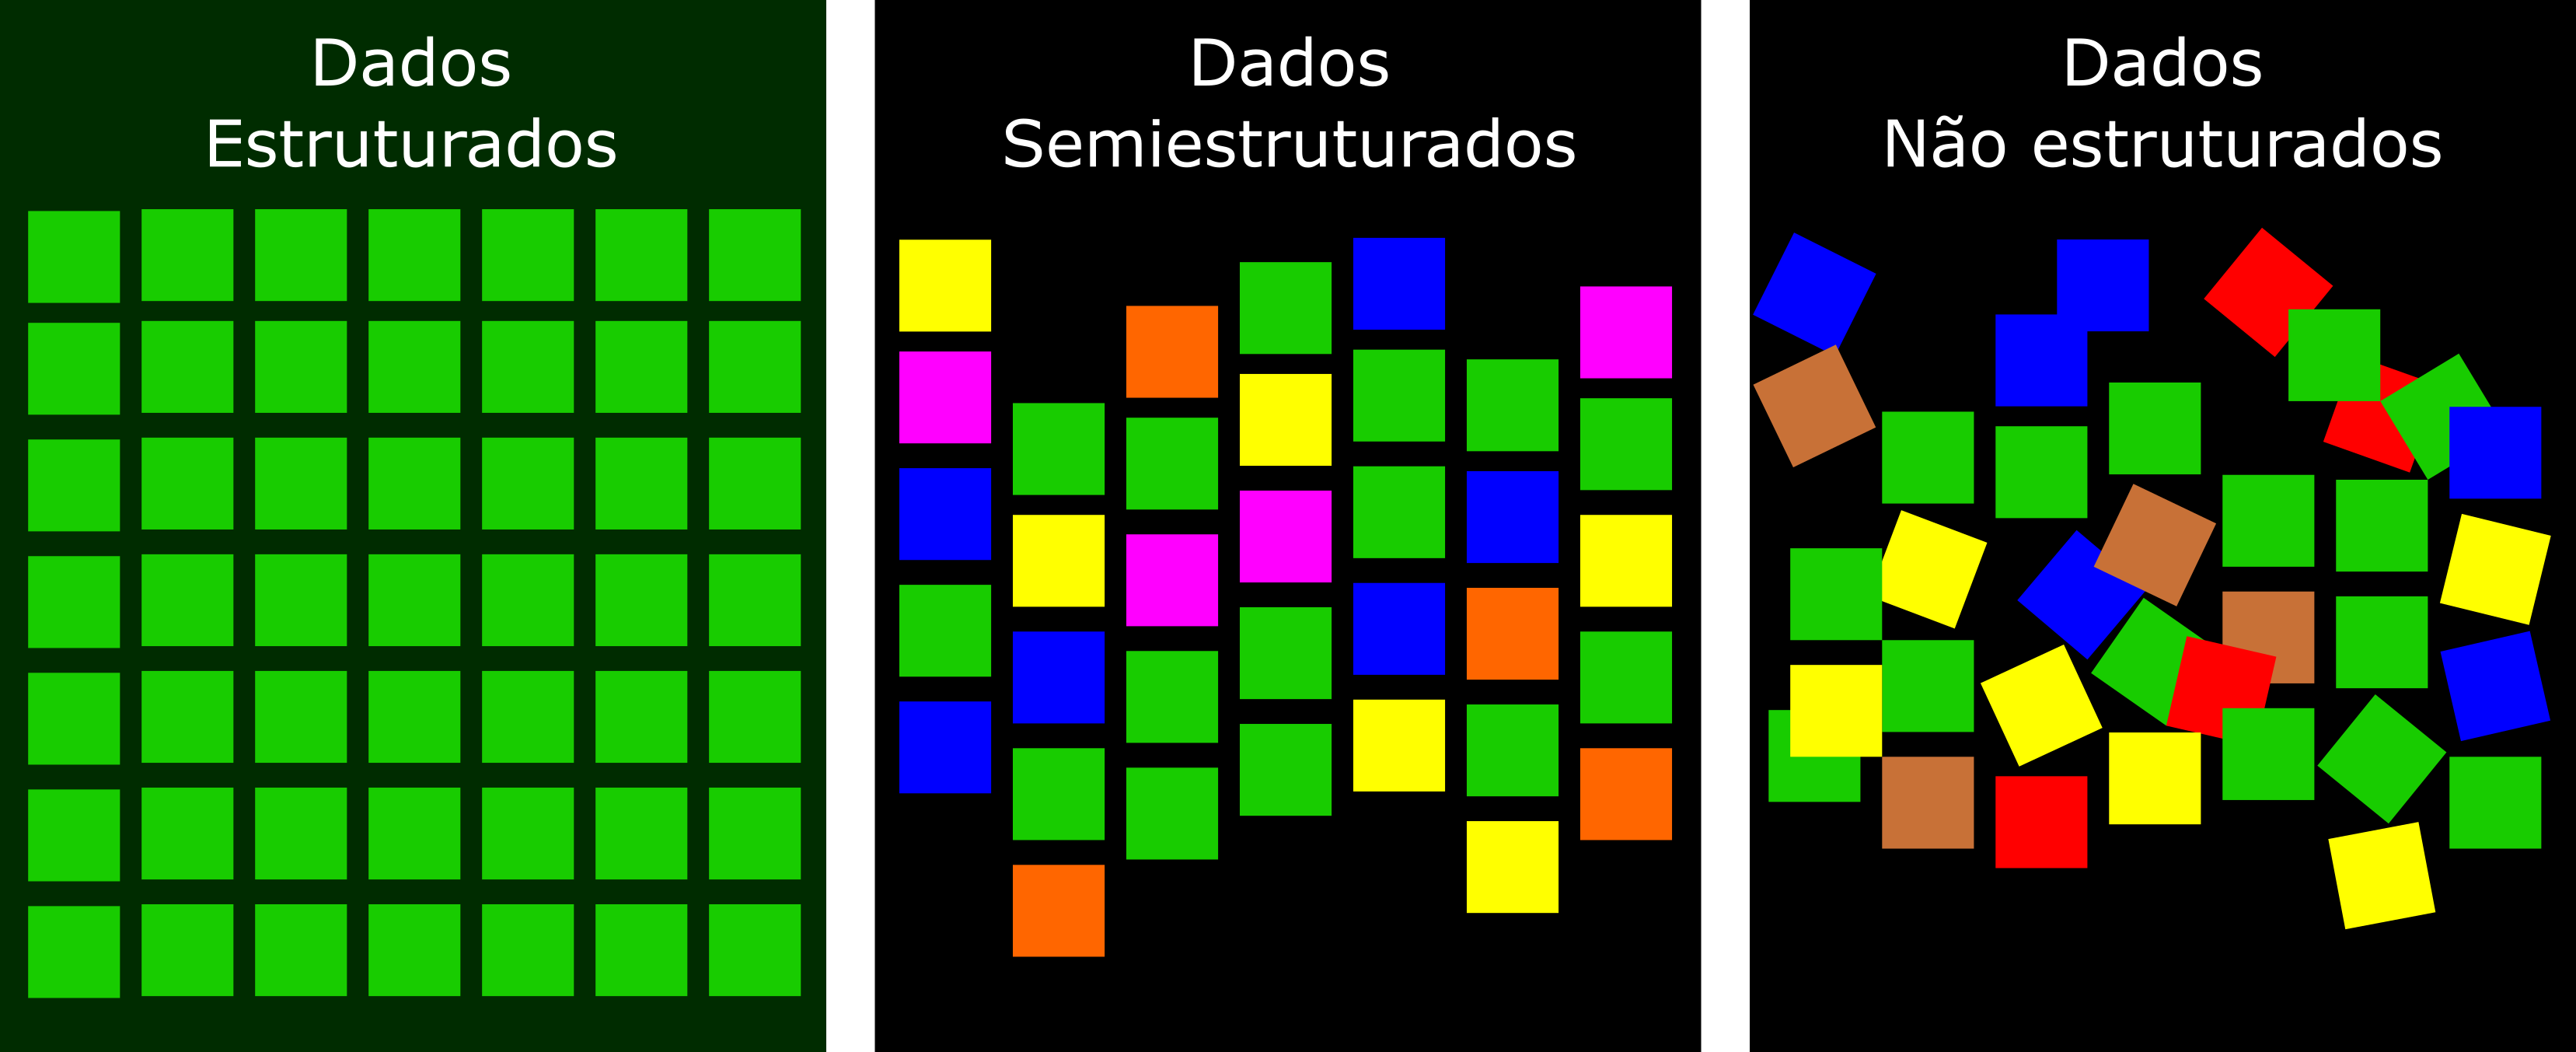
\includegraphics[width=0.9\textwidth]{figuras/dados.png}
		\label{fig:identificador_da_figura}
		\fonte{Autor}
	}
\end{figure}

\observacao{Observação/anotação para conversar com o orientador ou destacar importância.}

Utilize o comando \texttt{$\backslash$tachado\{\}} para tachar um texto. Exemplo: \tachado{comprar} adquirir.

Esse texto é um exemplo para \correcao{destaques de correção} a serem realizadas.

\subsection{Subseção}
\label{subsec:subseçao}
Bla bla bla
